\documentclass[letterpaper]{article}

\usepackage{natbib,alifeconf,xcolor,subcaption}  %% The order is important

% Automatic formatting of SI units
\usepackage[binary-units]{siunitx}

% Visible TODO notes
\newcommand{\todo}[1]{\textbf{\textsc{\textcolor{red}{(TODO: #1)}}}}
% *****************
%  Requirements:
% *****************
%
% - All pages sized consistently at 8.5 x 11 inches (US letter size).
% - PDF length <= 8 pages for full papers, <=2 pages for extended
%    abstracts.
% - Abstract length <= 250 words.
% - No visible crop marks.
% - Images at no greater than 300 dpi, scaled at 100%.
% - Embedded open type fonts only.
% - All layers flattened.
% - No attachments.
% - All desired links active in the files.

% Note that the PDF file must not exceed 5 MB if it is to be indexed
% by Google Scholar. Additional information about Google Scholar
% can be found here:
% http://www.google.com/intl/en/scholar/inclusion.html.


% If your system does not generate letter format documents by default,
% you can use the following workflow:
% latex example
% bibtex example
% latex example ; latex example
% dvips -o example.ps -t letterSize example.dvi
% ps2pdf example.ps example.pdf


% For pdflatex users:
% The alifeconf style file loads the "graphicx" package, and
% this may lead some users of pdflatex to experience problems.
% These can be fixed by editing the alifeconf.sty file to specify:
% \usepackage[pdftex]{graphicx}
%   instead of
% \usepackage{graphicx}.
% The PDF output generated by pdflatex should match the required
% specifications and obviously the dvips and ps2pdf steps become
% unnecessary.


% Note:  Some laser printers have a serious problem printing TeX
% output. The use of ps type I fonts should avoid this problem.


\title{Critical Exponent of Species-Size Distribution in Evolution}
\author{Chris Adami$^{1}$, Ryoichi Seki$^{1,2}$ \and Robel Yirdaw$^2$ \\
\mbox{}\\
$^1$California Institute of Technology, Pasadena, CA 91125 \\
$^2$California State University, Northridge, CA 91330 \\
adami@caltech.edu} % email of corresponding author

% For several authors from the same institution use the same number to
% refer to one address.
%
% If the names do not fit well on one line use
%         Author 1, Author 2 ... \\ {\Large\bf Author n} ...\\ ...
%
% If the title and author information do not fit in the area
% allocated, place \setlength\titlebox{<new height>} after the
% \documentclass line where <new height> is 2.25in



\begin{document}
\maketitle

\begin{abstract}
% Abstract length should not exceed 250 words
  aa
\end{abstract}

\section{Introduction}
dd

\section{Methods}
\subsection{Familiarity-driven navigation algorithms}
\begin{itemize}
    \item InfoMax
    \item PerfectMemory
\end{itemize}

\begin{figure}[t]
    \centering
    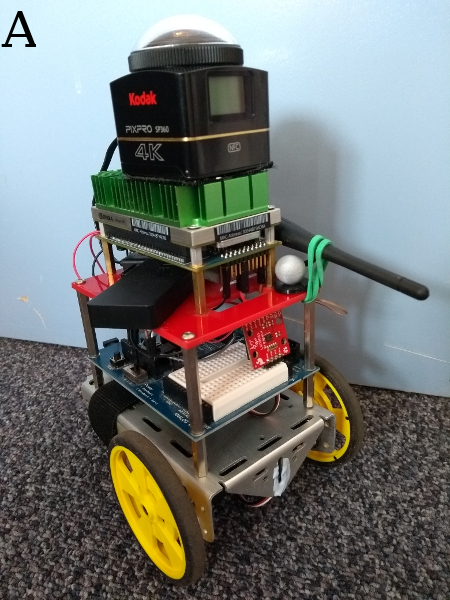
\includegraphics[width=2in]{figures/robot.jpg}
    \caption{Robot platform with onboard computation.}
    \label{fig:robot}
\end{figure}

\subsection{Robot platform}
\label{sec:robot_platform}
Our robot platform [10] shown in figure~\ref{fig:robot} is based on a Parallax ‘Shield-Bot’ chassis [?], with a Jetson TX1 embedded computer [?] mounted on top for additional onboard computation as well as additional batteries mounted underneath to power it. 
Finally the robot has a Kodak PixPro SP360 4K camera connected via USB to provide panoramic visual input.

\begin{figure}[t]
    \begin{subfigure}[b]{\columnwidth}
        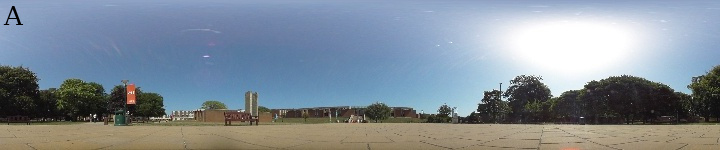
\includegraphics[width=\columnwidth]{figures/360_240.jpg}
        \caption{Unprocessed panoramic image}
    \end{subfigure}
    \begin{subfigure}[b]{\columnwidth}
        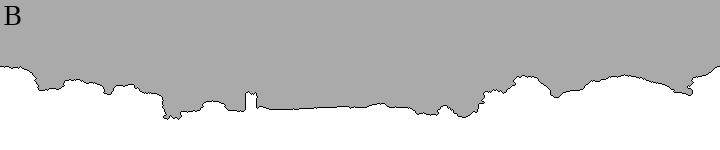
\includegraphics[width=\columnwidth]{figures/360_240_mask.png}
        \caption{Sky-segmented panoramic image}
    \end{subfigure}
    \caption{Example panoramic images from our database}
    \label{fig:database_images}
\end{figure}

\subsection{Image database}
\label{sec:image_database}
Using a Kodak PixPro SP360 panoramic camera, we recorded 195 images of the ‘Library Square’ at the University of Sussex (figure?). 
These were taken on a \SI{1.2}{\metre} grid, defined by square’s paving slabs. 
Alongside this reference grid, we also recorded videos from the same camera, mounted on the mobile robot described in the previous section, while we manually drove it along six routes of varying tortuosity across the square. 
As well as these videos, taken from the robot’s point-of-view, we simultaneously recorded the position of the robot using a camera mounted on a tripod. 
After synchronising these videos, we extracted the position of the robot over time using the Discriminative Correlation Filter Tracker with Channel and Spatial Reliability~\citep{Lukezic2018} implementation provided by OpenCV **CITE** and synchronised these positions with the video frames captured by the robot. 
\citet{Stone2014} showed that sky-segmented, binary images can be used for robust visual navigation and, while our robot does not have a suitable UV camera, by using the watershed segmentation algorithm~\citep{Beucher1979} with markers placed at the top and bottom of each image, we obtained automatically sky-segmented versions of all of the images in our dataset.
Figure~\ref{fig:database_images} shows some example images from this database.

\begin{figure*}[t]
    \centering
    \begin{subfigure}[t]{0.3\textwidth}
        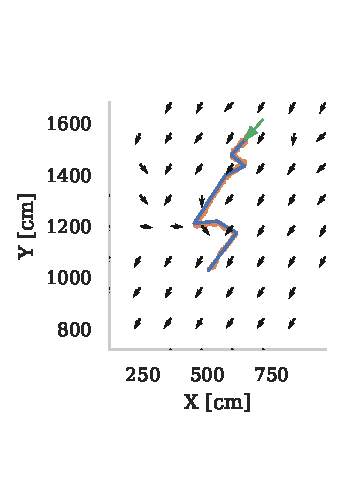
\includegraphics{figures/vector_field_route2_PerfectMemory_mask.eps}
        \caption{Simple route}
        \label{fig:vector_fields/route2_perfect_memory_mask}
    \end{subfigure}
    \begin{subfigure}[t]{0.3\textwidth}
        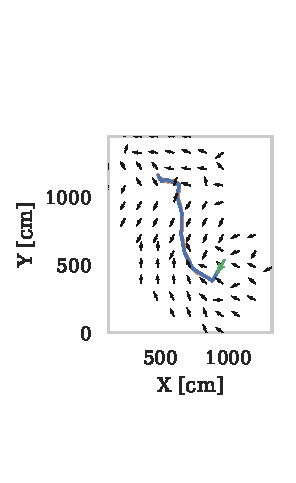
\includegraphics{figures/vector_field_route5_PerfectMemory_mask.eps}
        \caption{Longer route where visual aliasing occurs in the middle section}
        \label{fig:vector_fields/route5_perfect_memory_mask}
    \end{subfigure}
    \begin{subfigure}[t]{0.3\textwidth}
        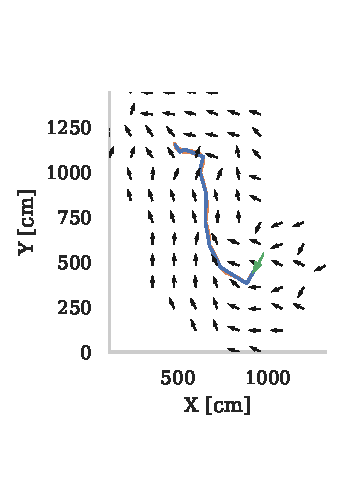
\includegraphics{figures/vector_field_route5_PerfectMemoryConstrained_mask.eps}
        \caption{By only considering rotated views within 90° of the route, visual aliasing can be avoided}
        \label{fig:vector_fields/route5_perfect_memory_constrained_mask}
    \end{subfigure}
    
    \caption{Vector fields showing the directions an agent, trained on a route, would move at each point within 4m of the route using a Perfect Memory algorithm with the skyline extracted using the watershed algorithm. 
    Orange lines shows data from our camera-based tracking of the robot and blue shows the version simplified using the Ramer-Douglas-Peucker algorithm~\citep{Ramer1972}}
    \label{fig:vector_fields}
\end{figure*}

\begin{figure}[t]
    \begin{subfigure}[b]{\columnwidth}
        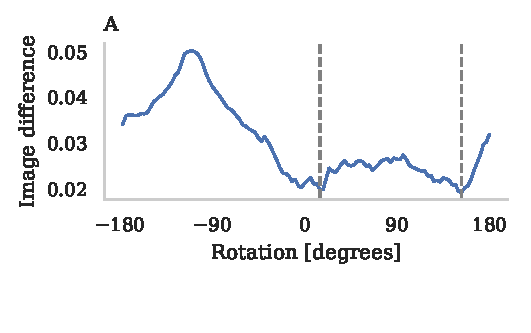
\includegraphics[width=\columnwidth]{figures/alias_ridf.eps}
        \caption{Rotational Image Difference function}
    \end{subfigure}
    
    \begin{subfigure}[b]{\columnwidth}
        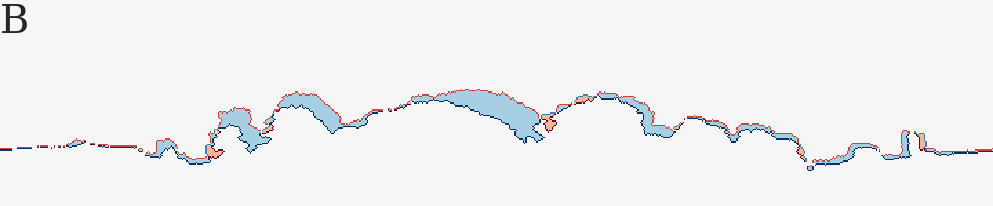
\includegraphics[width=\columnwidth]{figures/image_diff_bad.png}
        \caption{Difference image with visual aliased route image}
    \end{subfigure}
    
    \begin{subfigure}[b]{\columnwidth}
        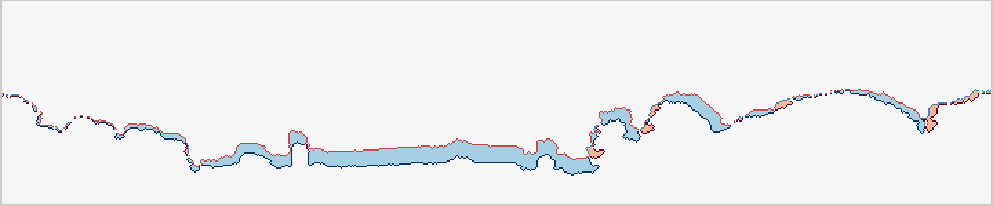
\includegraphics[width=\columnwidth]{figures/image_diff_good.png}
        \caption{Difference image with correct route image}
    \end{subfigure}
    \caption{Analysis of aliasing shown in figure~\ref{fig:vector_fields/route5_perfect_memory_mask}.
    Using grid image taken at (\SI{600}{\metre}, \SI{720}{\metre}.) }
\end{figure}

\begin{figure*}[t]
    \centering
    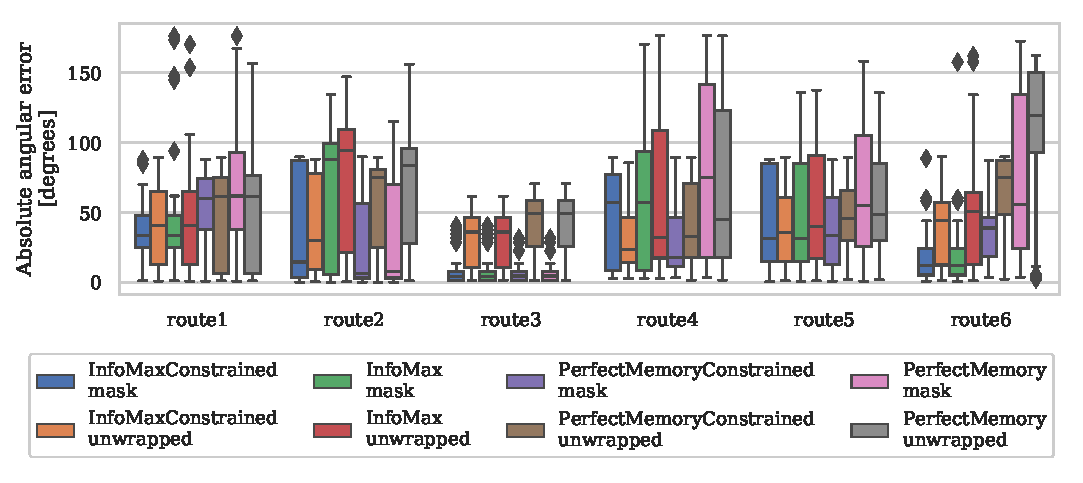
\includegraphics{figures/route_benchmark.eps}
    \caption{Performance of different algorithms on each of the 6 routes. \todo{decide on consistent names for routes}}
    \label{fig:route_benchmark}
\end{figure*}

\section{Results}
\subsection{Image database}
We trained both the InfoMax and Perfect Memory on each of the six routes in our dataset and calculated the familiarity against the images at each grid point within \SI{4}{\metre} of the trained route. 
To find the direction a robot would move when placed at each location, we rotated the grid image taken at that point through \SI{\pm 180}{\degree} and found the most familiar direction. 
Figure~\ref{fig:vector_fields} shows some example vector fields resulting from plotting this direction at each location. 
While the vector field suggests that the route shown in Figure~\ref{fig:vector_fields/route2_perfect_memory_mask} would be recapitulated successfully, in the middle section of the route shown in Figure~\ref{fig:vector_fields/route5_perfect_memory_mask}, errors occur.
\todo{figure showing of best match, RIDF, difference image etc}
However, if we were recapitulating the route using a real robot, these false-positive matches could be eliminated and computation could be saved by not scanning the full \SI{\pm 180}{\degree}. 
If we simulate this using our grid of images by only considering matches within \SI{\pm 90}{\degree} of the heading of the nearest section of the route (calculated based on the simplified version), as shown in Figure~\ref{fig:vector_fields/route5_perfect_memory_constrained_mask}, the performance is much improved.

\begin{figure}[t]
    \centering
    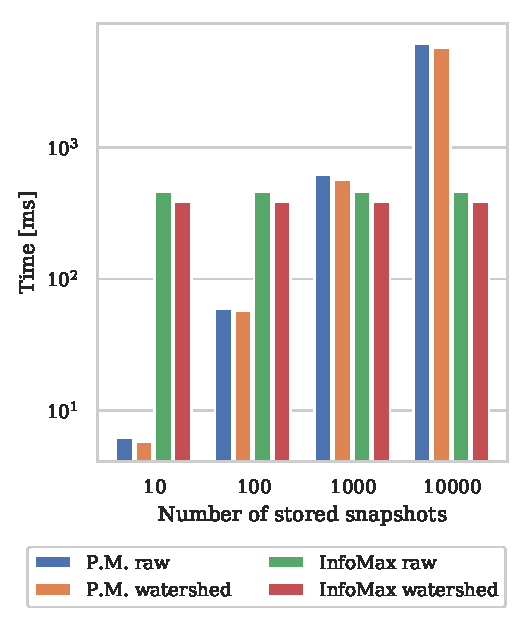
\includegraphics{figures/jetson_test_performance.eps}
    \caption{Performance of visual navigation algorithms running on Jetson TX1. Reported times are measured using .}
    \label{fig:jetson_test_performance}
\end{figure}

\subsection{Performance of algorithm}
In the previous section, we showed that these simple insect-inspired algorithms are capable of robustly extracting heading direction through dynamic natural scenes. 
However, in order to deploy these algorithms on a real robot with constrained on board processing, their performance is important. 

\begin{figure}[t]
    \centering
    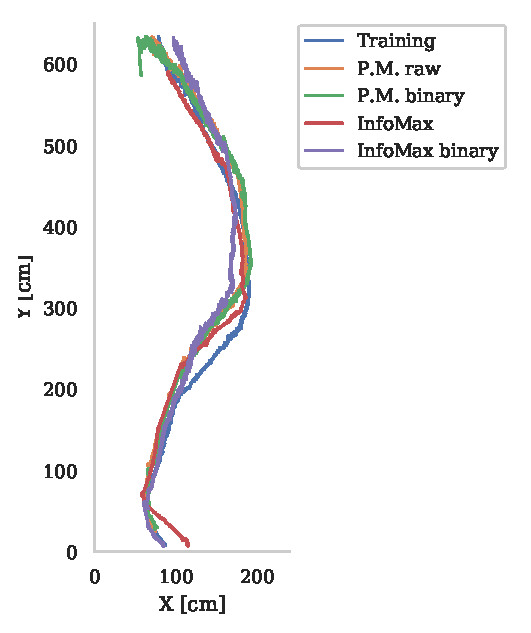
\includegraphics{figures/robot_paths.eps}
    \caption{Reconstructed paths of autonomous robot during training and testing using each algorithm.}
    \label{fig:robot_paths}
\end{figure}


\subsection{Autonomous robot}
Using the same implementations of InfoMax and the Perfect Memory from our Brains-on-Board Robotics **ref** library, we built a simple application which can recapitulate learned routes on the robot described in section~\ref{sec:robot_platform} by running the following simple algorithm every \SI{500}{\milli\second} (based on the performance for 1000 images established in the previous section):
\begin{enumerate}
    \item Capture and unwrap a panoramic image.
    \item Perform one of the image processing steps described in section~\ref{sec:image_database}.
    \item Using either the InfoMax or Perfect Memory algorithm, calculate the familiarity with the processed image ‘in-silico’ when rotated through \SI{\pm 90}{\degree}°.
    \item Find the orientation with the highest familiarity - if it is within \SI{4}{\degree} (**CHECK**) drive forwards for the next \SI{500}{\milli\second}, otherwise turn in the correct direction to align with the image.
\end{enumerate}
We tested our robot in an outdoor environment 

\section{Discussion}
\begin{itemize}
    \item how/why SLAM is the obvious alternative
    \item General limitations of monocular SLAM
\end{itemize}
Typically, visual SLAM implementations extract features such as SURF or SIFT which require several hundreds of milliseconds to extract per frame~\citep{Bay2006}. 
This makes such implementations impractical to use in real-time, especially on constrained mobile platforms. 
However, more recent SLAM implementations such as FLaME~\citep{Greene2017} have been shown to run on autonomous quadrotors in only around \SI{10}{\milli\second} per frame. 
While this is significantly faster than our current InfoMax implementation, \citet{Greene2017} were using a much more powerful Intel CPU on their quadrotor (\citet{Biddulph2018} measure it as being $5\times$ faster). 
Furthermore, when \citet{Baddeley2012} first demonstrated InfoMax for visual navigation, they used input images with around half the number of pixels used here. 
Because the time taken to calculate the matrix-vector product required for equation**REFERENCE** scales quadratically, using input images with half the number of pixels would quarter the time taken to evaluate equation**REFERENCE**.

\section{Conclusions}
ss
\section{Acknowledgements}
This work was funded by the EPSRC (Brains on Board project, grant number EP/P006094/1).
We would also like to thank Daniil Sakhapov for his work collecting the `library square' database of images, Alex Dewar for developing the BoB robotics framework and Norbert Domcsek for assisting with the data collection for this paper. 

\footnotesize
\bibliographystyle{apalike}
\bibliography{alife} % replace by the name of your .bib file


\end{document}
